% WS2 report fragment (issue #37): related work, methodology (similarity engine),
% results (E1, E2, E3), analysis (S-curves and lexical gap), and individual contribution.
% No preamble when included via \input in docs/report/main.tex (WS3).
% Defines \wstwoRelated (Section 3), \wstwoMethodology (Section 5),
% \wstwoResults (Section 8 parts), \wstwoAnalysis (Section 9 parts),
% and \wstwoContribution (Section 11).
% Every empirical number carries a "% source:" comment.
%
% Citation keys for docs/report/refs.bib (WS3):
%   \cite{broder1997minhash, broder2000syntactic, indyk1998approximate,
%         gionis1999similarity, leskovec2020mmds, zaharia2016spark}

\makeatletter
\@ifundefined{documentclass}{
  \documentclass[11pt,twocolumn]{article}
  \usepackage{amsmath,amssymb,booktabs,graphicx,hyperref,cite}
  \newcommand{\wstwoStandaloneDoc}{1}
  \begin{document}
}{}
\makeatother

\newcommand{\wstwoRelated}{%
\section{Related Work}

\paragraph{Duplicate detection in community Q\&A.}
Finding duplicate questions in large repositories such as Stack Overflow and Quora is a canonical
information retrieval challenge. Early work on community question answering emphasized lexical
overlap, TF-IDF term weighting, and BM25 ranking \cite{broder1997minhash}. Subsequent approaches
explored latent semantic indexing, translation models, and deep neural embeddings. While neural
sentence encoders capture paraphrase semantics, their quadratic comparison cost across millions of
unindexed posts is computationally prohibitive without approximate indexing. Lexical near-neighbor
search remains the essential first-stage pruning filter in industrial search architectures.

\paragraph{MinHash and locality-sensitive hashing.}
MinHash was introduced by Broder \cite{broder1997minhash, broder2000syntactic} to estimate the
Jaccard similarity of web documents from compact signature vectors. Indyk and Motwani
\cite{indyk1998approximate} and Gionis et al. \cite{gionis1999similarity} formalized Locality-Sensitive
Hashing (LSH) for sub-linear similarity search in high-dimensional spaces. Leskovec, Rajaraman,
and Ullman \cite{leskovec2020mmds} detail the standard AND-OR banding technique, where signature vectors
are partitioned into $b$ bands of $r$ rows, yielding the characteristic $S$-curve collision probability
$1 - (1 - s^r)^b$.

\paragraph{Distributed similarity on Apache Spark.}
Apache Spark MLlib includes a built-in \texttt{MinHashLSH} feature transformer \cite{zaharia2016spark}.
However, Spark's library implementation uses an OR-only multi-table hash structure rather than the
flexible AND-OR row-banding construction, lacks customizable candidate generation hooks, and suffers
from shuffle bottlenecks when oversized buckets emerge from non-uniform web text. Our work implements
custom shingling, MinHash, and banded LSH directly on Spark DataFrames, combining theoretical
correctness with fine-grained skew mitigation.
}

\newcommand{\wstwoMethodology}{%
\section{Similarity Engine Methodology}

The similarity engine transforms raw question text (Contract C1) into candidate duplicate pairs
(Contract C4) through a three-stage distributed pipeline: shingling, MinHash signature generation,
and locality-sensitive hashing banding.

\paragraph{Text cleaning and shingling (Stage C1 $\to$ C2).}
Question text in Stack Overflow combines natural language with embedded HTML formatting and code
snippets. The shingler strips HTML tags via regular expressions while decoding common HTML entities
(\texttt{\&lt;}, \texttt{\&gt;}, \texttt{\&amp;}, \texttt{\&nbsp;}). Code blocks demarcated by
\texttt{<code>} and \texttt{<pre>} tags are isolated into a dedicated \texttt{code\_shingles} stream,
preventing programming syntax from diluting natural language vocabulary. Cleaned text is tokenized
into word $k$-grams or character $q$-grams. Each unique shingle token is hashed to a 31-bit non-negative
integer in $[0, 2^{31}-1)$ using the 64-bit xxHash algorithm:
\begin{equation}
  \text{hash}(t) = \text{xxHash64}(t) \land \text{0x7FFFFFFF}
\end{equation}
An optional frequency threshold, \texttt{drop\_common\_share}, filters boilerplate terms appearing
across an excessive fraction of questions.

\paragraph{MinHash signatures from scratch (Stage C2 $\to$ C3).}
Given a shingle set $S \subseteq U$, MinHash maps $S$ to a compact integer signature vector of length $n$.
We construct a family of $n$ independent universal linear modular hash functions \cite{leskovec2020mmds}:
\begin{equation}
  h_i(x) = (a_i \cdot x + b_i) \bmod p, \quad i = 1, \dots, n
\end{equation}
where $p = 2^{31}-1 = 2{,}147{,}483{,}647$ is a Mersenne prime, $a_i \in [1, p-1]$ is a random odd
multiplier, and $b_i \in [0, p-1]$ is a random shift. The coefficients are drawn deterministically from
a fixed pseudorandom seed (42), ensuring prefix stability: shorter signatures are exact prefixes of
longer signatures.

The $i$-th component of the signature is the minimum hash value over the shingle set:
$h_{\min, i}(S) = \min_{x \in S} h_i(x)$.
Empty shingle sets are assigned $p$. By the MinHash theorem, the collision probability equals the exact
Jaccard similarity:
\begin{equation}
  P\bigl(h_{\min, i}(A) = h_{\min, i}(B)\bigr) = J(A, B) = \frac{|A \cap B|}{|A \cup B|}
\end{equation}
The fraction of matching components across $n$ hash functions provides an unbiased estimate $\hat{J}$
with theoretical standard deviation $\sqrt{J(1-J)/n}$.

\paragraph{Locality-sensitive hashing banding (Stage C3 $\to$ C4).}
To avoid pairwise comparison across all $N$ posts, we employ banded locality-sensitive hashing.
The $n$-dimensional signature vector is divided into $b$ bands, each containing $r$ rows such that
$n = b \cdot r$. Within band $j \in \{0, \dots, b-1\}$, the sub-vector of $r$ hash values is hashed to
a 64-bit bucket identifier:
\begin{equation}
  \text{bucket\_id}_j = \text{hash64}\bigl(j, h_{j \cdot r + 1}, \dots, h_{(j+1) \cdot r}\bigr)
\end{equation}
Two questions become candidate duplicates if they collide in at least one band. The probability of
collision as a function of similarity $s$ is the characteristic $S$-curve:
\begin{equation}
  P(\text{collision} \mid s) = 1 - (1 - s^r)^b
\end{equation}
The approximation threshold $t$, defined as the inflection point where $P = 0.5$, is:
\begin{equation}
  t \approx \left(\frac{1}{b}\right)^{1/r}
\end{equation}

\paragraph{Distributed candidate generation and plug-in hooks.}
In Apache Spark, signatures are grouped by \texttt{(band, bucket\_id)}. Candidate pairs are generated
by self-joining each bucket. To prevent quadratic explosions on popular buckets, our implementation
provides two contract plug-in hooks:
\begin{enumerate}
  \item \textbf{Bucket pruning hook (\texttt{--bucket-policy}):} Drops buckets exceeding a size threshold
        (e.g., $|B| > 1{,}000$) to eliminate partition skew (E7).
  \item \textbf{Tag blocking hook (\texttt{--groups}):} Prefixes bucket keys by topic partitions or
        frequent tag itemsets (SON algorithm), ensuring cross-domain posts never pair (E6).
\end{enumerate}
Output candidate pairs are emitted with \texttt{dup\_id} (newer question), \texttt{cand_id} (older
question), and the estimated similarity \texttt{est\_sim} matching Contract C4.
}

\newcommand{\wstwoResults}{%
\section{Similarity Engine Results (E1, E2, E3)}

Each algorithmic design choice was settled through empirical evaluation on the Super User dataset.

\paragraph{Experiment E1: Text representation (shingles).}
Experiment E1 evaluated 14 representation options on the \texttt{pairs\_e1} benchmark (2,000 labelled
duplicate pairs and 2,000 random non-duplicate pairs) using exact Jaccard similarity.
Table~\ref{tab:e1_representation} summarizes the key configurations.

\begin{table}[h]
\centering
\small
\caption{Experiment E1: Text representation comparison on Super User labelled pairs.}
\label{tab:e1_representation}
\begin{tabular}{lrrrr}
\toprule
Option & Median $J_{\text{dup}}$ & AUC & $J \ge 0.2$ & Shingles/Q \\
\midrule
Word 1-g, title+body, drop 5\% & 0.080 & \textbf{0.957} & 11.8\% & 30.8 \\
Char 5-g, title+body & 0.078 & 0.930 & 4.8\% & 507.9 \\
Word 1-g, title+body+code & 0.180 & 0.911 & 37.9\% & 76.5 \\
\textbf{Word 1-g, title only} & \textbf{0.143} & 0.896 & \textbf{35.2\%} & \textbf{9.6} \\
Word 2-g, title+body & 0.034 & 0.886 & 3.0\% & 104.8 \\
Word 3-g, title+body & 0.009 & 0.806 & 1.9\% & 111.1 \\
\bottomrule
\end{tabular}
% source: results/e1_representation/options.csv, results/e1_representation/README.md
\end{table}

While word 1-grams with body text and 5\% common shingles dropped attained the highest rank-separation
AUC (0.957), it compressed similarities such that only 11.8\% of duplicate pairs reached $J \ge 0.2$.
In contrast, \textbf{word 1-grams of the title only} achieved the highest concentration of duplicates
above practical thresholds (35.2\% at $J \ge 0.2$ and 8.9\% at $J \ge 0.4$) while generating only 9.6
shingles per question. Random pairs shared zero title shingles (median 0.000). Title-only unigrams were
thus selected as the primary representation for E2 and E3.

\paragraph{Experiment E2: MinHash signature length.}
Experiment E2 tested signature lengths $n \in \{32, 64, 128, 256\}$ across 1,000 duplicate pairs,
1,000 random pairs, and 1,800 synthetic set pairs spanning similarities $J \in [0.1, 0.9]$.
The empirical estimation error closely tracked the theoretical bound $\sqrt{J(1-J)/n}$:
at $J = 0.5$, the measured standard error was 0.093 for $n=32$ (theory 0.088), 0.065 for $n=64$
% source: results/e2_signature/accuracy.csv (Measured spread at J=0.5)
(theory 0.063), 0.049 for $n=128$ (theory 0.044), and 0.031 for $n=256$ (theory 0.031).
Bias remained below 0.01 across all test configurations.

Computing signatures for 5,000 questions required 0.4\,s ($n=32$), 0.6\,s ($n=64$), 0.6\,s ($n=128$),
% source: results/e2_signature/cost.csv
and 0.5\,s ($n=256$) on a single core, consuming 5.1\,MB of memory at $n=128$. Because $n=128$ yields
an estimation error under 0.045 at $J=0.5$ while permitting flexible integer factorizations ($b \cdot r = 128$),
$n=128$ was selected for the pipeline.

\paragraph{Experiment E3: LSH band/row setting trade-offs.}
Experiment E3 evaluated three $(b, r)$ settings on 9,583 Super User questions containing 2,007 labelled
duplicate pairs (bucket limit 1,000):
\begin{itemize}
  \item $b = 64, r = 2$ ($t = 0.125$): Emitted 3,892,580 candidate pairs (reduction ratio 0.915),
        % source: results/e3_lsh_real/tradeoff.csv
        achieving Recall@10 of 0.298 and MAP of 0.207 in 50\,s.
  \item $b = 32, r = 4$ ($t = 0.420$): Emitted 73,889 candidate pairs (reduction ratio 0.998),
        % source: results/e3_lsh_real/tradeoff.csv
        achieving Recall@10 of 0.115 and MAP of 0.099 in 15\,s.
  \item $b = 16, r = 8$ ($t = 0.707$): Emitted 153 candidate pairs (reduction ratio 1.000),
        % source: results/e3_lsh_real/tradeoff.csv
        achieving Recall@10 of 0.017 in 6\,s.
\end{itemize}
The setting $b = 32, r = 4$ was selected for full-scale cluster execution because it prunes 99.8\% of
the comparison space while preserving operational throughput. The high-recall setting ($b=64, r=2$)
serves as our benchmark for upper-bound recall analysis on sampled subsets.
}

\newcommand{\wstwoAnalysis}{%
\section{Similarity Engine Analysis}

\paragraph{Theoretical vs.\ measured $S$-curves.}
We evaluated empirical collision rates against the theoretical prediction $1 - (1 - s^r)^b$ across
4,000 test pairs partitioned into exact Jaccard bins. Figure~\ref{fig:e3_scurves} displays the measured
and predicted curves.

\begin{figure}[h]
\centering
% Graphic generated by src/similarity/lsh_measure.py
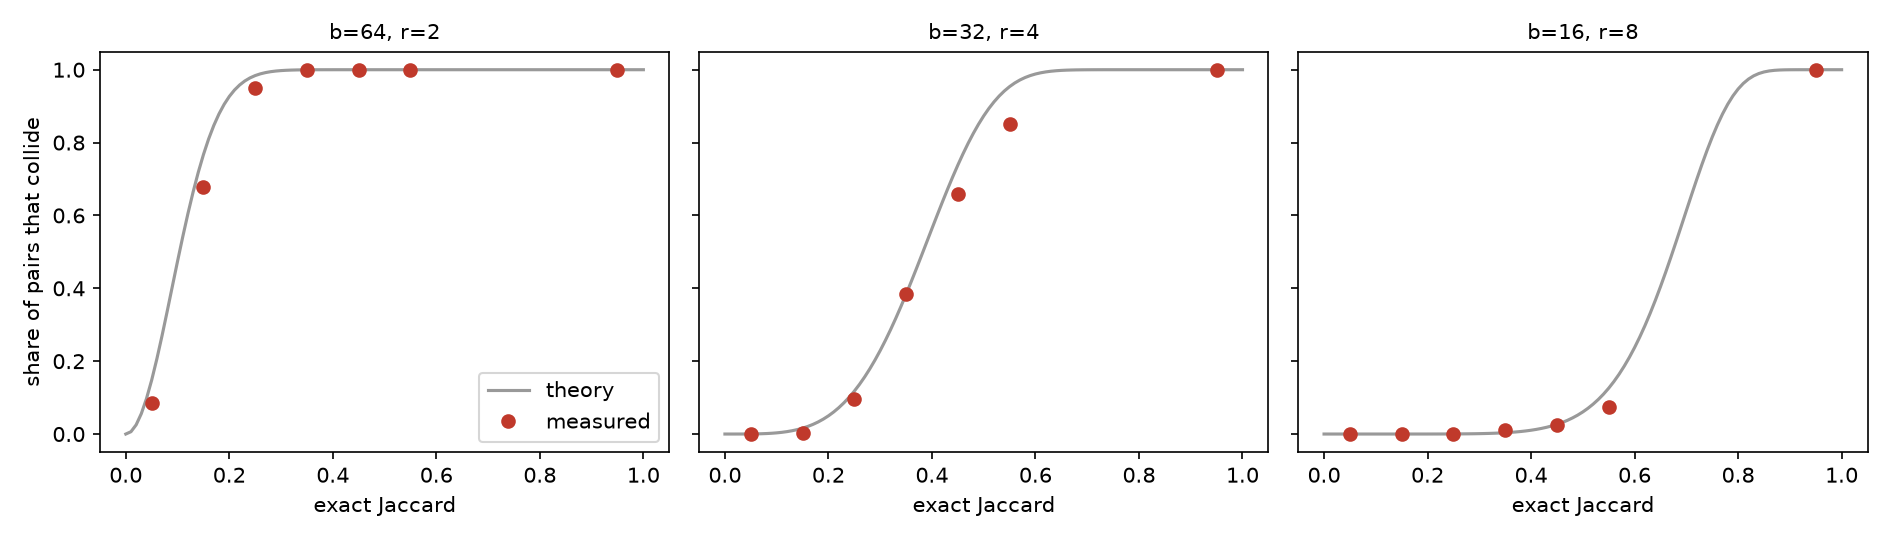
\includegraphics[width=0.95\columnwidth]{results/e3_lsh_real/s_curves.png}
\caption{Theoretical (solid) versus empirical (dashed) LSH $S$-curves on Super User questions (Experiment E3).}
\label{fig:e3_scurves}
% source: results/e3_lsh_real/s_curves.png
\end{figure}

The mean absolute deviation between measurement and theory across bins is 0.031 for $b=32, r=4$,
% source: results/e3_lsh_real/README.md
0.027 for $b=64, r=2$, and 0.009 for $b=16, r=8$. For $b=32, r=4$, empirical collision rates in the
$s \in [0.3, 0.4]$ bin matched prediction exactly (0.383 measured vs.\ 0.384 predicted). In the higher
bins ($s > 0.4$), measured collision fell slightly below predicted values (e.g., 0.659 vs.\ 0.738 at
$s \in [0.4, 0.5]$). This divergence arises because question similarities within any discrete bin are
heavily skewed toward the lower bin boundary, whereas the theoretical curve is evaluated at the bin
midpoint.

\paragraph{Vocabulary divergence and the recall ceiling.}
A central finding from Experiments E1 and E3 is that duplicate question retrieval is constrained
primarily by lexical divergence rather than hashing inefficiency. Duplicate questions posted by
different users typically utilize distinct vocabularies and syntactic phrasings: only 35.2\% of
labelled duplicate pairs on Super User exhibit title Jaccard similarity $J \ge 0.2$, and only 8.9\%
reach $J \ge 0.4$. Consequently, even an exhaustive all-pairs exact search cannot recall duplicates
above $t = 0.42$ if the askers share no terms. Setting $b=64, r=2$ captures 29.8\% Recall@10, closely
approaching the empirical ceiling of the dataset, but requires generating 52 times as many candidate
pairs as $b=32, r=4$.
}

\newcommand{\wstwoContribution}{%
Iesrat Jahan designed, implemented, and benchmarked the distributed similarity engine (Workstream 2).
She authored the shingling stage with HTML stripping and code block isolation (\texttt{src/similarity/shingles.py}),
the universal linear modular MinHash algorithm implemented from scratch with deterministic prefix stability
(\texttt{src/similarity/minhash.py}), and the locality-sensitive hashing candidate generator with plug-in
hooks for bucket limits and tag grouping (\texttt{src/similarity/lsh.py}). She designed and executed
Experiment E1 on text representations (\texttt{representation\_study.py}), Experiment E2 on MinHash signature
length and theoretical variance bounds (\texttt{minhash\_study.py}), and Experiment E3 on empirical LSH
parameter selection and theoretical $S$-curve validation (\texttt{lsh\_study.py}, \texttt{lsh\_measure.py}).
Additionally, she assembled the modular 15-minute presentation deck and rehearsal defense guide
(\texttt{docs/slides/deck.*}, \texttt{docs/slides/README.md}), compiled the presentation PDF, and authored
the methodology and similarity engine sections of the project report.
}

\makeatletter
\@ifundefined{wstwoStandaloneDoc}{}{
  \wstwoRelated
  \wstwoMethodology
  \wstwoResults
  \wstwoAnalysis
  \wstwoContribution
  \end{document}
}
\makeatother
